\documentclass[blue]{beamer}
\usepackage{beamerthemeFrankfurt} 
\usecolortheme{rose}
\usepackage{amsmath}
\usepackage{amssymb}
%\usepackage{cite} % never use with beamer 
\usepackage{hyperref}
\usepackage{latexsym}
\usepackage{graphicx}
\usepackage{multirow}
\usepackage{adjustbox}
\makeatletter
\newcommand{\removelatexerror}{\let\@latex@error\@gobble}
\makeatother
\makeatletter
\let\@@magyar@captionfix\relax
\makeatother
\usepackage{url}
\newtheorem{assumption}{Assumption}
\usepackage{setspace}
\setbeamertemplate{itemize/enumerate body begin}{\small}
\usepackage{tabulary}
\usepackage[algo2e,linesnumbered,ruled,vlined]{algorithm2e} 
%\usepackage{algpseudocode,algorithm,algorithmicx}
\setbeamercolor{title}{fg=red!80!black,bg=red!20!white}
 %   \setbeamerfont{block title}{size=\scriptsize} change block title font size
%\setbeamerfont{title}{shape=\itshape,family=\rmfamily}
%\usetheme{Warsaw} % brings shadowness
\usefonttheme{professionalfonts} % font theme
\newtheorem{answeredquestions}[theorem]{Answered Questions}
\usepackage[figuresright]{rotating}
\usepackage{subfig}
\graphicspath{{images/}{use/}{infersent/}}
%\usefonttheme[onlysmall]{structurebold} %%%small fonts in the navigation bars are a bit hard

\title{Online Similarity Learning with Feedback for Invoice Line Item Matching}
\author[Chandresh]{Chandresh Kumar Maurya \\  Assistant Professor\\ }
\institute{E\"otv\"os Lor\'and University, Budapest, Hungary}
\begin{document}
\maketitle
% without [fragile], any {verbatim} code gets mysterious errors.


%\begin{frame}
%\frametitle{Research Contribution}
%So far, I have worked on the following problems:
%\begin{itemize}
%\item Anomaly Detection in Big Data (Ph.D. Topic)
%\item Creative Tagline Generation for Product Advertisement
%\item Prediction of Invoice Payment Status in Account Payable Business Process.
%\item Similarity Learning with Feedback for Invoice Line Item Matching
%\end{itemize}
%
%\end{frame}

\begin{frame}[shrink=20]
\footnotesize
\frametitle{Publications (Journals)}

\begin{enumerate} 
\item 

C. Maurya; D. Toshniwal; G. Venkoparao, ``Distributed Sparse Class-Imbalance Learning and its Applications," in {\bf IEEE Transactions on Big Data} , vol.PP, no.99, pp.1-1
https://doi.org/10.1109/TBDATA.2017.2688372

\item
Chandresh Kumar Maurya, Durga Toshniwal, Gopalan Vijendran Venkoparao, Online sparse class imbalance learning on big data, {\bf Neurocomputing}, Volume 216, 5 December 2016, Pages 250-260, ISSN 0925-2312, http://doi.org/10.1016/j.neucom.2016.07.040. (IF 3.317)

\item 
Chandresh Kumar Maurya, Durga Toshniwal, Large-Scale Distributed Sparse Class-Imbalance Learning with Application to Anomaly Detection,  {\bf Information Sciences}, Volume 456, 4 May 2018, Pages 1-12, ISSN 0020-0255, Elsevier, https://doi.org/10.1016/j.ins.2018.05.004 (IF 4.832)

\item   Creative Tagline Generation Framework for Product Advertisement, Chandresh Kumar Maurya et al.,  in {\bf IBM Journal of Research \& Development}) (SCIE IF 0.6)
\item {\bf Online Similarity Learning with Feedback for Invoice Line Item Matching} (submitted to IEEE TKDE)
\end{enumerate}
\end{frame}

\begin{frame}[shrink=20]
\footnotesize
\frametitle{Publications (Conferences/Workshops)}

\begin{enumerate} 
\item 
Prediction of Invoice Payment Status in Account Payable Business Process. Tarun Tater, Sampath Dechu, Senthil Mani, and Chandresh Kumar Maurya, {\bf International Conference on Service-Oriented Computing (ICSOC)} 2018, China.

\item
 Anomaly Detection via Distributed Sparse Class-Imbalance Learning. Chandresh Kumar Maurya, Durga Toshniwal, and  Vishal Agarwal, ( presented in \textcolor{red}{International Conference on Machine Learning, ICML 2016} workshop on Anomaly detection, NY, USA)


\item
Online Anomaly Detection via Class-Imbalance Learning, Chandresh Kumar Maurya and Durga Toshniwal,  in  {\bf International Conference on Contemporary Computing (IC3)} , organised jointly by JIIT Noida and University of Florida, USA, Sep 2015.

\item
 Anomaly Detection in Nuclear Power Plant Data using Support Vector Data Description, Chandresh Kumar Maurya and Durga Toshniwal, in  IEEE TechSym at IIT Kharagpur, Feb 2014.

\item  Fuzzy Inference System for Internet Traffic Load Forecasting, Chandresh Kumar Maurya and Sonajharia Minz. In the Proceedings of National Conference of Computing \& Communications (NCCCS)-
2012. DOI:10.1109/NCCCS.2012.6413010. .

\item
Anomaly Detection in Streaming Data using Online Non-negative Matrix Factorization, Chandresh Kumar Maurya, Arun Chauhan and Durga Toshniwal, poster presentation at International workshop on machine learning \& Text analytic(MLTA 2013), South Asian University, New Delhi.  (\textcolor{red}{Best  presentation Award})
\end{enumerate}
\end{frame}

\begin{frame}[shrink=20]
\footnotesize
\frametitle{Patents While @IBM}

\begin{enumerate} 
\item A System and Method for Automatic Adjustment of Brightness of Mobile Devices based on Visual Sight ({\bf under FILE})

\item A System and Method for Recommending Popular Features for a Product based on Crowd-source Reviews of the Product and Competitor Product  ({\bf Rated search-2 by IBM, under search}) 


\item A System and Method for Finding Best Accommodation using Deep Asthetic Features in Multimodal Data from Social Networks. ({\bf Defensive publication})

\item A System and Method for Automatic  Compliance Checking in Clinical Process using Deep Multi-task Learning. ({\bf  Defensive publication})

\item A system and Method for Similarity Learning with Heterogeneous Catalogues and Taxonomies for Invoice and PO Line Item Matching (under review).
\item  An Intelligent and Proactive Reminder System using Multi-Modal Data through AI (under review).

\item 
A System and Method for Consistency Verification of Product’s Information on E-commerce Portals (under review).
\end{enumerate}
\end{frame}

\begin{frame}
\frametitle{Outline}
  \tableofcontents %[pausesections]
\end{frame}
%====================================================
\section{Introduction}

\begin{frame}{Similarity Learning with Feedback for Invoice Line Item Matching}

\begin{block}{Procure to Pay process}
\begin{figure}
\centering
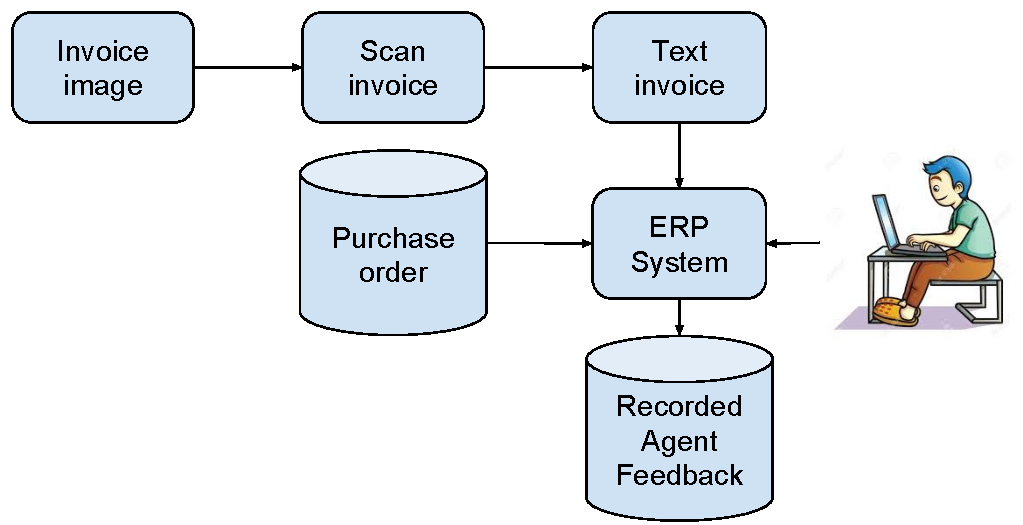
\includegraphics[height=4cm]{sdm_p2p.pdf}
\caption{Invoice line item matching in P2P business process}
\label{fig:invoice}
\end{figure}

\end{block}
\end{frame}

\section{The Problem}

\begin{frame}{The problem}

 \begin{table}[]
\caption{An example of line item matching}
\label{lineitem}
\resizebox{\columnwidth}{!}{%
\begin{tabular}{|l|l|}
\hline
Invoice                           & PO                                                                                                                                        \\ \hline \hline


TRES 739mL CD KER Smooth  & \begin{tabular}[c]{@{}l@{}}1. TRES 0.739L CD KER Smth\\ 2. Tres Soya Smooth Conditioner 150 gm\end{tabular} \\ \hline


5x200ml Fruit Juice 100\% - Tropicana, Apple  & \begin{tabular}[c]{@{}l@{}}1. Tropicana 100\% Apple Juice -  1L\\ 2. Fruit Juice 500ml - Tropicana, Custard Apple\end{tabular} \\ \hline
Battery Distilled Water Replacement      & \begin{tabular}[c]{@{}l@{}}1. Battery Maintenance Services\\ 2.  Battery Warranty extension\end{tabular}                              \\ \hline
\end{tabular}}
\end{table}
\end{frame}


\begin{frame}{Our Contribution}
\begin{itemize}
 \itemsep0em
\item  Two approaches are proposed to match descriptions
using domain knowledge captured in the user’s
feedback. First approach learns similarity rank when
recorded users feedback has relative ranking of description matches and second approach uses binary
classification when users’ recorded feedback is absolute match/no-match between pair of descriptions.
\item To circumvent the issue of hierarchical relationship
among items in the invoice and PO line items, we
present an algorithm that makes use of product tax-
onomy and catalog.
\item Proposed approaches are evaluated on real-world
description datasets e.g. invoice data from internal clients, publicly available product description datasets and compare the results with the state-of-the-art approaches applied to natural language sentences and show limitations of the existing work. Additionally, we also evaluate the proposed approachs using different kinds of description representations such as character n-gram (n=2 to 5), directly encoding the description assuming them as sentence via
pre-trained models from Infersent [4] and Google’s
universal sentence encoder. [5].
\end{itemize}

\end{frame}

\section{Related work}

\begin{frame}{Related Work}

\begin{itemize}
\item In \cite{chechik2010large}, the author present an online relative similarity learning task for images. They learn a metric $W$ based on the triples of the images within the passive-aggressive learning framework \cite{crammer2006online}

\item In \cite{liu2015computing}, the author uses support vector regression with various features such as WordNet-Based features, corpus-based features, Word2Vec-based feature, Alignment-based features, and Literal-based features to predict the similarity between short English sentences.

\item In \cite{kashyap2016robust} proposes a robust distributional word similarity component that combines the LSA and ML augmented data from several linguistic resources.

\item In \cite{kutiyanawala2018towards,hu2018reinforcement} the author propose matching query to items in the product catalog.

\end{itemize}
\end{frame}


\section{Our Approach}

\begin{frame}{Proposed Algorithm}

\begin{figure}
\centering
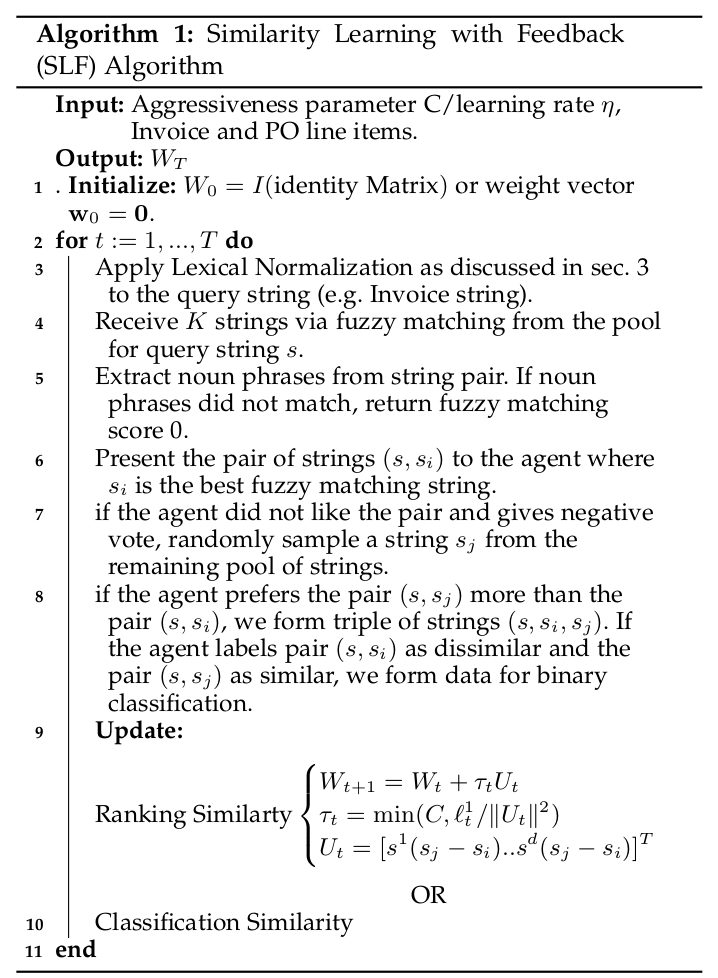
\includegraphics[height=8cm]{algo.png}
\caption{Similarity learning with feedback algorithm}
\label{fig:algo}
\end{figure}
\end{frame}

\begin{frame}{Online Metric Similarity Learning}
We want to learn a function $f(\cdot, \cdot)$ that assigns high score to pairs $(s, s_j)$ than the pair $(s, s_i)$ whenever the agent prefers $(s, s_j)$ more than $(s, s_i)$. Assume that the function $f$ has a bilinear form shown in \eqref{bilinear}.
    \begin{equation}\label{bilinear}
        f_W(s_i, s_j) := s_i^TWs_j
    \end{equation}
    where the matrix $W \in R^{d\times d}$. 
Our objective is to find the function $f(\cdot,\cdot)$  such that all the triplet strings satisfy the contraint in \eqref{const}.
    \begin{equation}\label{const}
        f_W(s,s_j) \geq f_W(s,s_i) +1
    \end{equation}
\end{frame}


\begin{frame}{Contd...}
The constraint in \eqref{const} leads to the following loss function.
    \begin{equation}\label{hinge}
        \ell^1_t(s,s_i,s_j) = \max(0,1-f_W(s,s_j)+f_W(s,s_i))
    \end{equation}
    
  Following  \cite{crammer2006online}, we can plug the above loss in passive-agressive algorithm as shown in \eqref{prob}.
    \begin{equation}\label{prob}
\begin{aligned}
& W_{t+1} &= \text{argmin}_W \|W-W_t\|_{fro} + C\xi \\
& \text{s.t.} &\ell^1_t(s,s_i,s_i) \leq \xi \hspace{0.5cm} \text{and}\hspace{0.5cm} \xi \geq 0
\end{aligned}
\end{equation}
\end{frame}
\section{Experimental Results}

\begin{frame}{Datasets}
\begin{table}[htbp]
\centering
\caption{Summary of  datasets  used in the experiment}
\label{data}
\resizebox{\columnwidth}{!}{%
\begin{tabular}{|l|l|l|l|}
\hline
Dataset & \#Train &\# Test  & \#Features   \\ \hline \hline
Invoice & 370 & 184 & 3649\\\hline
Amazon Electronics & 9368 &4683 & 35327\\\hline
Amazon Automative& 21107 & 10553 & 40123\\\hline
Amazon Home&21887 & 10943 &46453\\\hline
Flipkart & 9417 & 4708 & 19400\\\hline
SNLI & 121895& 60947&55956\\\hline
SICK & 3865 & 1932 & 18379\\\hline
STS & 1426 & 713 & 16110\\\hline
\end{tabular}}
\end{table}
\end{frame}

\begin{frame}{Preprocessing}
Invoice data  consists of invoice strings ($s$). We have the corresponding PO strings ($s_j$) a.k.a second string) as well. Since, there is no third string ($s_i$) available, we manually curated and generated third string  from the second one (PO string) under the following assumption so that third string is less similar to the invoice string compared to the PO string. The following rules are derived during manual curation of the invoice data:
\begin{enumerate}
    \item Common antonyms such as men vs women.
    \item Small delta Numeric addition or deletion - for second string
    \item Large delta Numeric addition or deletion - for third string
    \item Replace Brand names, if applicable
    \item Replace Product names, if applicable
    \item String Manipulation such as insertion/deletion/substitution of random character and shuffle words
\end{enumerate}

\end{frame}

\begin{frame}{Contd...}
 An example of string triple from invoice data look like as follows:
\begin{itemize}
    \item [$s$:]12z Dove Men US 2in1 FRts
   \item [$s_j$:] 11z Dove Men US 2in1 Frts 
 \item [$s_i$:] 12z Dove women US 2in1 Shampoo
\end{itemize}
\end{frame}

\begin{frame}{Experimental Testbed and Setup}
Proposed approach is compared against the following methods:
\begin{itemize}
\item Cosine Similarity
\item Li's method \cite{li2006sentence}
\item  UMBC \cite{han2013umbc_ebiquity}
\item  Siamese method \cite{neculoiu2016learning}

\end{itemize}•


\end{frame}

\begin{frame}{Learning behavior of SLFR}
\begin{figure}
\subfloat[Invoice]{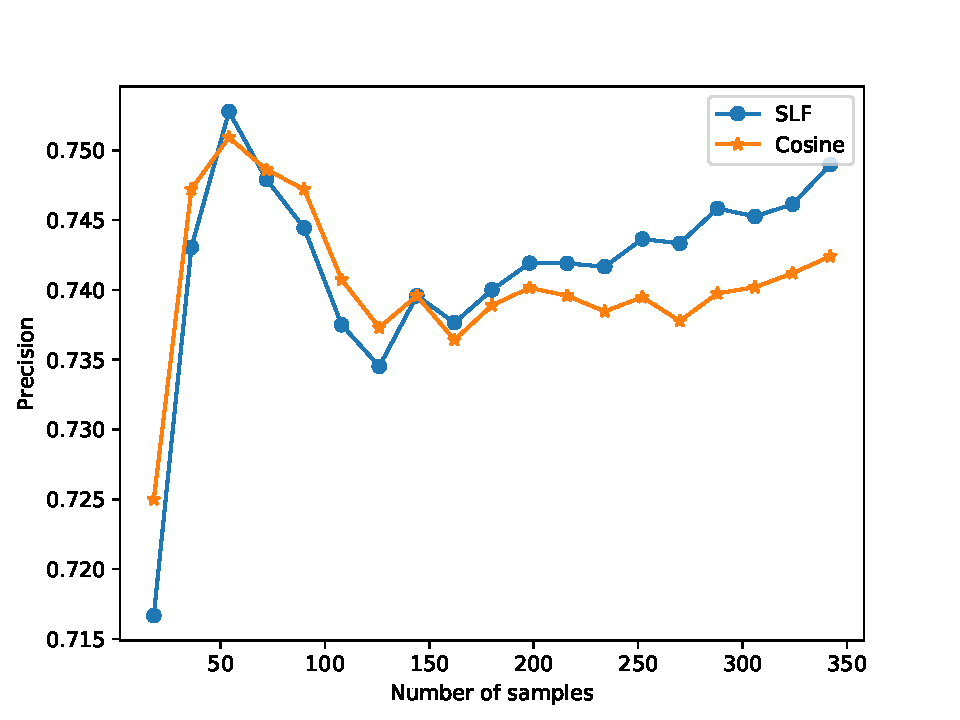
\includegraphics[width=3cm, height=3cm]{invoice_npztrain.pdf}}
\subfloat[Amazon Electronics]{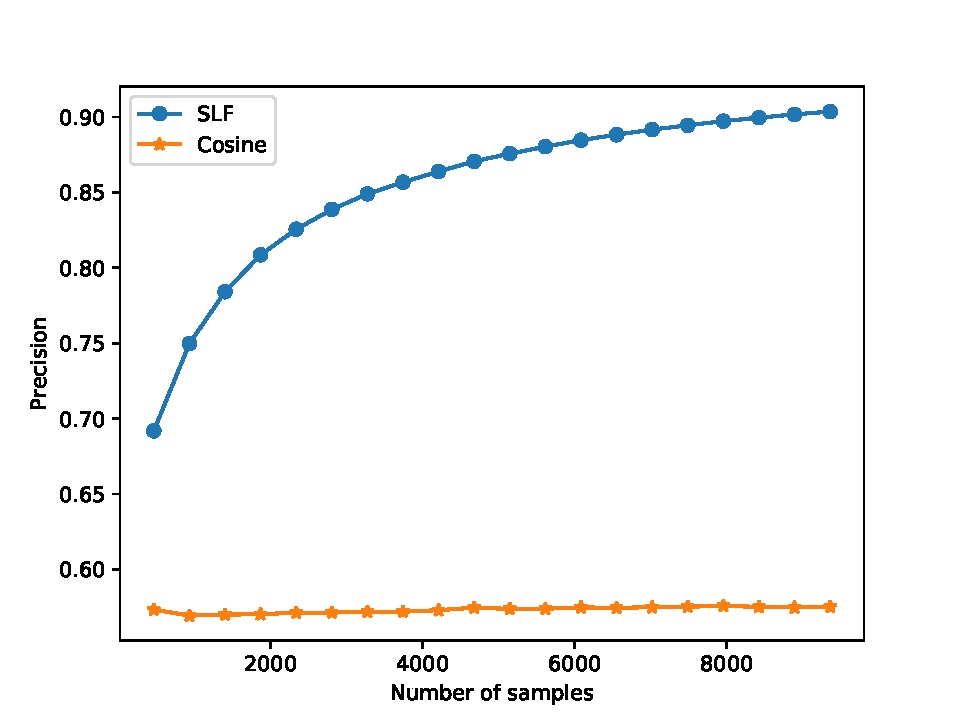
\includegraphics[width=3cm, height=3cm]{amazondata_electronics_npztrain.pdf}} 
\subfloat[Amazon Automotive]{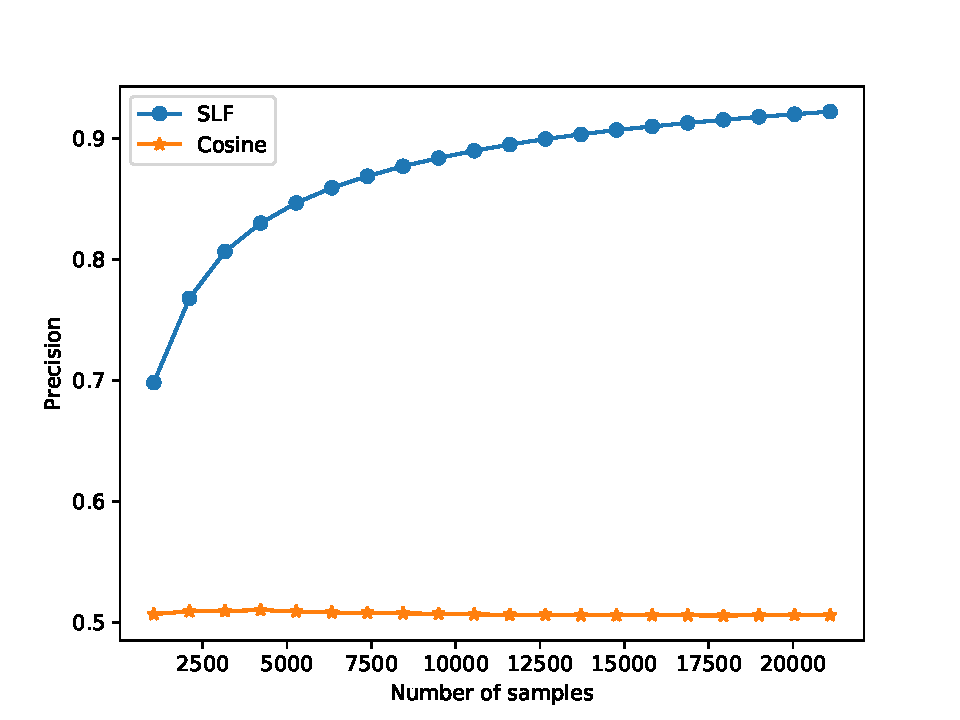
\includegraphics[width=3cm, height=3cm]{amazondata_automotive_npztrain.pdf}}
\subfloat[Amazon Home]{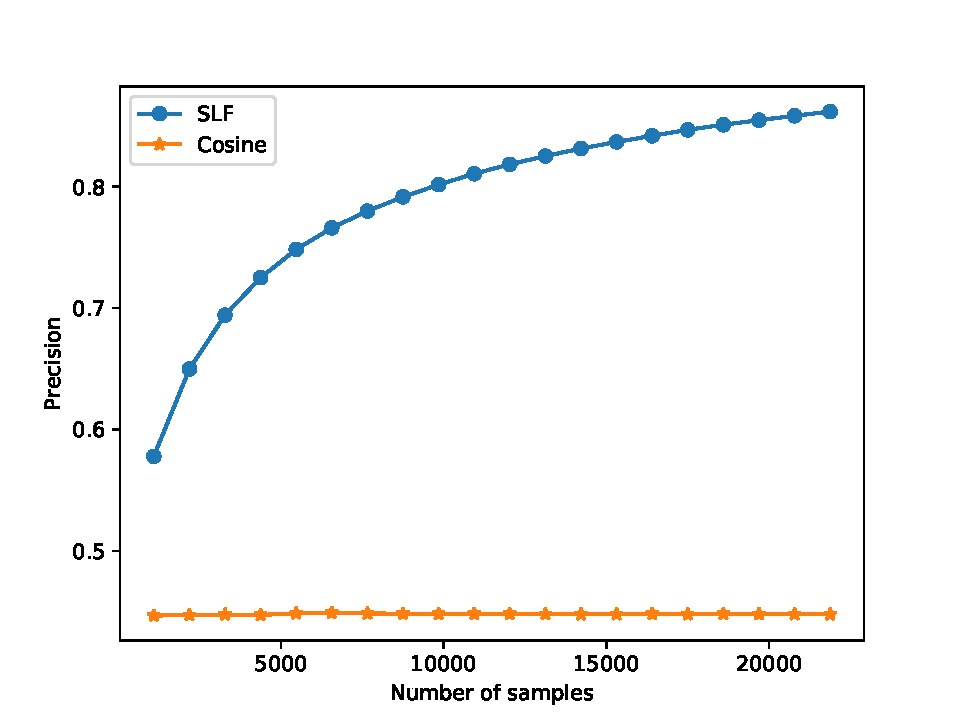
\includegraphics[width=3cm, height=3cm]{amazondata_home_npztrain.pdf}}

\caption{Evaluation of online average of \emph{recall} over various benchmark data sets. (a) invoice (b) Amazon electronics (c) Amazon Automotive (d) Amazon Home } 
\label{fig:recall}
\end{figure}

\end{frame}
\begin{frame}{Contd...}
\begin{figure}

\subfloat[Flipkart]{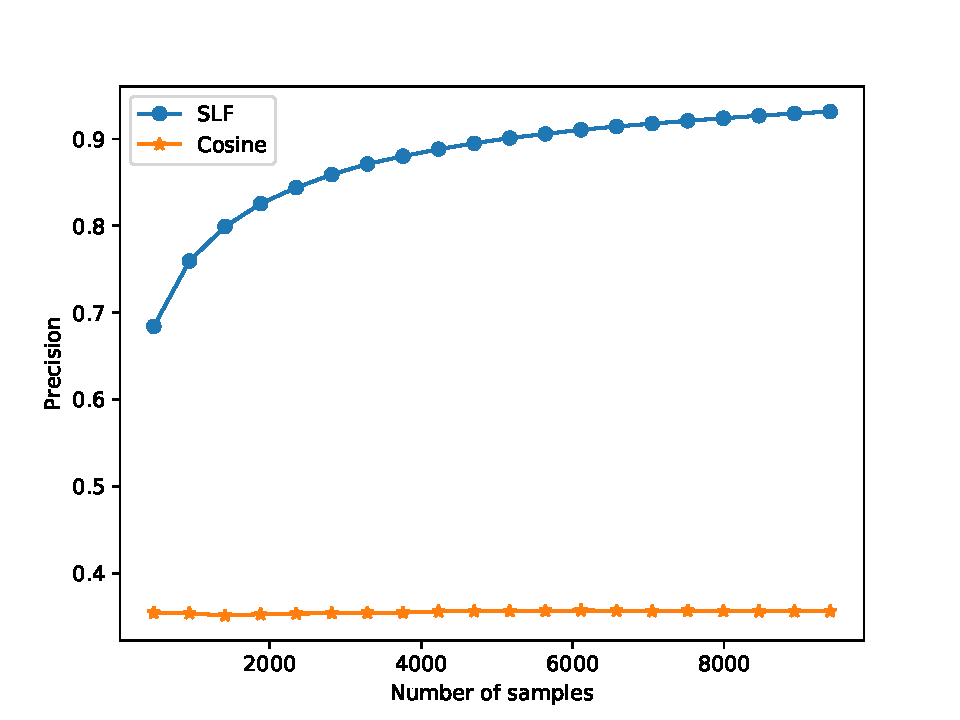
\includegraphics[width=3cm, height=3cm]{flipkart_out_npztrain.pdf}}
\subfloat[SNLI]{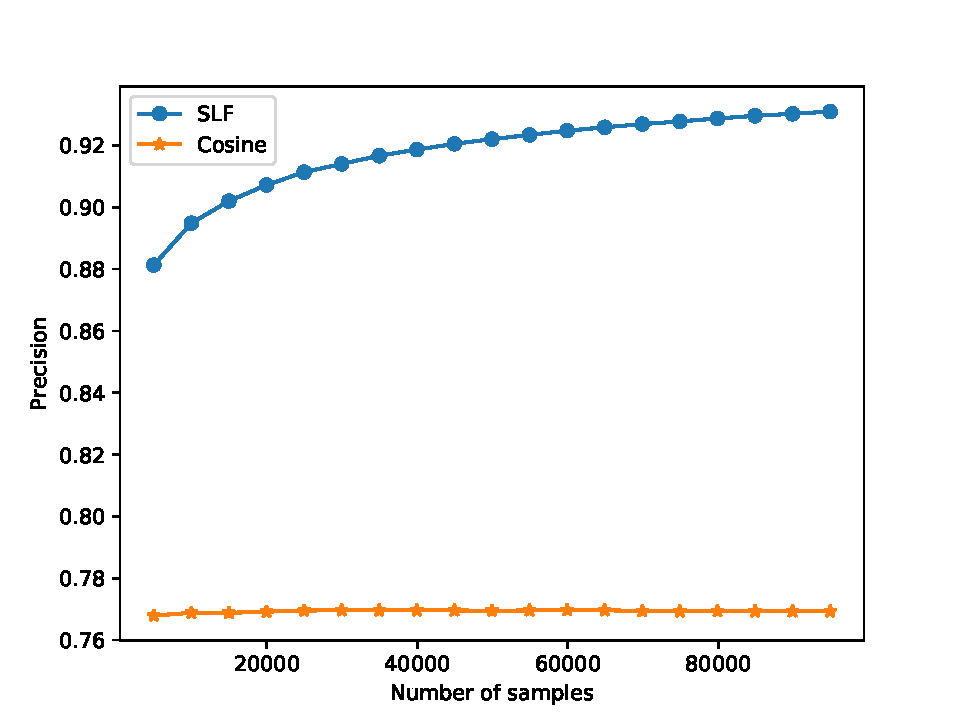
\includegraphics[width=3cm, height=3cm]{snli_npztrain.pdf}}
\subfloat[SICK]{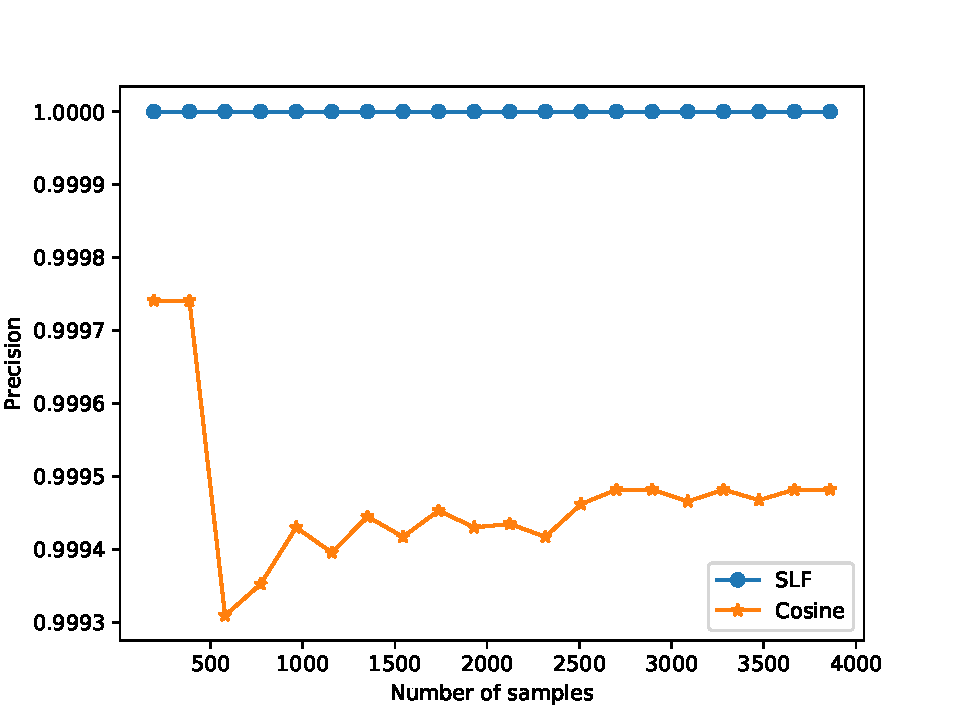
\includegraphics[width=3cm, height=3cm]{sick_npztrain.pdf}} 
\subfloat[STS]{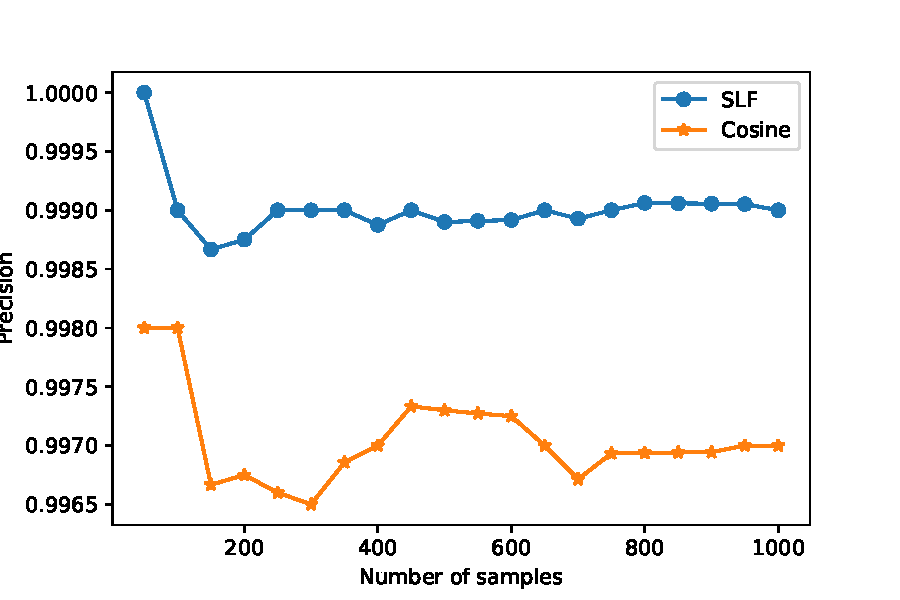
\includegraphics[width=3cm, height=3cm]{sts_npztrain.pdf}}
\caption{Evaluation of online average of \emph{recall} over various benchmark data sets. (a) Flipkart (b) SNLI (c) SICK (d) STS } 
\label{fig:recall}
\end{figure}

\end{frame}

\begin{frame}[shrink=10]{Generalization Performance of SLFR}
\begin{table}[]
\caption{Evaluation on the test data (average precision over 20 runs) using three encoding schemes}
\label{encoding}
\centering
\begin{tabular}{|l|l|l|l|}
\hline
 \backslashbox[]{Data}{Encoding}   & Tf-idf & Infersent & USE   \\ \hline
Invoice                                            &\textbf{77.77}  & 62.22     & 62.77 \\ \hline
Amazon Electronics                                 & \textbf{80.70}  & 65.62     & 75.53 \\ \hline
Amazon Automotive                                  & \textbf{90.75}  & 82.77     & 50.61 \\ \hline
Amazon Home                                        & \textbf{86.35}  & 82.62     & 77.04 \\ \hline
Flipkart                                           & 86.83  & \textbf{87.74}     & 84.57 \\ \hline
SNLI                                               & 94.34  &  94.36         &\textbf{ 99.19} \\ \hline
SICK                                               & \textbf{99.89}  & 95.15     & 99.58 \\ \hline
STS                                                &\textbf{99.34}  & 95.60     & 98.40 \\ \hline
\end{tabular}
\end{table}
\end{frame}

\begin{frame}[shrink=10]{Comparative Performance Evaluation of SLFR}
\begin{table}[]
\caption{Comparative evaluation of average precision on test data }
\label{tab:recall}
\begin{tabular}{|p{2cm}|l|l|l|l|p{1cm}|}
\hline
\backslashbox[]{Data}{Algo}  & SLFR  & Cosine & Li    & DKPRo & Siamese \\ \hline
Invoice                                            &\textbf{77.77} & 73.33  & 65.64 & 52.17 & 13.61   \\ \hline
Amazon Electronics                                 & \textbf{80.70} & 58.29  & 40.90 & 41.34 & 9.64    \\ \hline
Amazon Automotive                                  & \textbf{90.75} & 51.31  & 39.64 & 40.64 & 9.71    \\ \hline
Amazon Home                                        & \textbf{86.35} & 45.70  & 40.01 & 35.56 & 10.78   \\ \hline
Amazon Flipkart                                    & \textbf{86.83} & 28.35  & 24.67 & 27.71 & 5.60    \\ \hline
SNLI                                               & \textbf{94.34} & 76.92  & 75.61 & 20.08 & 23.63   \\ \hline
SICK                                               & 99.89 & \textbf{99.94}  & 99.94 & 79.34 & 9.98    \\ \hline
STS                                                & \textbf{99.34} & 99.20  & 99.21 & 79.34 & 8.23    \\ \hline
\end{tabular}
\end{table}

\end{frame}


\begin{frame}[shrink=10]{Comparative Performance Evaluation of SLFC}
\begin{table}[]
\centering
\caption{Average Precision, Recall and F-score from GradientBoost classifer on tf-idf, Infersent and USE encoded data}
\label{class:ngram}
\begin{tabular}{|l|l|l|l|l|l|l|l|l|l|}
\hline
                   & \multicolumn{3}{c|}{Tf-df}   & \multicolumn{3}{c|}{Infersent} & \multicolumn{3}{c|}{USE}     \\ \hline
Dataset            & Precision & Recall & F-score & Precision  & Recall  & F-score & Precision & Recall & F-score \\ \hline
Invoice            & 0.29      & 0.29   & 0.29    &{\bf 0.30}       & {\bf 0.30}    & {\bf 0.30}    & 0.27      & 0.27   & 0.27    \\ \hline
SICK               & 0.81      & 0.81   & 0.81    & {\bf 0.83}       & {\bf 0.85}    & {\bf 0.85}    & {\bf 0.85}      & {\bf 0.85}   & {\bf 0.85}    \\ \hline
STS                &{\bf 0.86}      & {\bf 0.85}   & {\bf 0.85}    & 0.60       & 0.60    & 0.60    & 0.73      & 0.73   & 0.73    \\ \hline
SNLI               & 0.73      & 0.73   & .073    & 0.75       & 0.75    & 0.75    & {\bf 0.83}      & {\bf 0.83}   & {\bf 0.83}    \\ \hline
Amazon Automotive  & 0.76      & 0.75   & 0.75    & {\bf 0.88}       & {\bf 0.87}    & {\bf 0.87}    & 0.47      & 0.47   & 0.46    \\ \hline
Amazon Electronics & {\bf 0.72}      & {\bf 0.72}   &{\bf  0.72}    & 0.55       & 0.55    & 0.55    & 0.51      & 0.51   & 0.51    \\ \hline
Amazon Home        & 0.74      & 0.74   & 0.73    & {\bf 0.89}       & {\bf 0.89}    &{\bf  0.89}    & 0.57      & 0.57   & 0.57    \\ \hline
Flipkart           & 0.87      & 0.86   & 0.86    & {\bf 0.93}       & {\bf 0.93}    & {\bf 0.93}    & 0.71      & 0.71   & 0.71    \\ \hline
\end{tabular}
\end{table}
\end{frame}



\section{Future Research Plan}

\begin{frame}{Research Problems}
\begin{itemize}
\item [Problem 1] Finding Best Accommodation using Deep Aesthetic features in Multimodal Data from Social Networks

\item [Problem 2] Recommending Popular Features for a Product based on Crowd-source Reviews of the Product and Competitor Product  

\item [Problem 3] Intelligent Reminder System using Multimodal Data

\item [Problem 4] Generating image advertisement given a catchy tagline
%
%\item [Problem 4] Automating traffic light

\end{itemize}•
\end{frame}

%\section{Teaching plan}
%
%\begin{frame}{Teaching plan}
%Some of the basic and advanced subjects I would like to teach are:
%\begin{itemize}
%\item Design and analysis of algorithms
%\item Data Structures
%\item Linear algebra
%\item Probability \& Statistics
%\item Matrix Calculus
%
%\end{itemize}
%Advanced courses
%\begin{itemize}
%\item Machine Learning/Data Science
%\item Reinforcement learning
%\item Convex/non-convex optimization
%\item General AI
%\item NLP
%\item IR
%
%\end{itemize}
%
%\end{frame}



\begin{frame}[allowframebreaks]{Bibliography}
\fontsize{8pt}{7.2}\selectfont
\bibliographystyle{apalike}
\bibliography{./TKDE}
\end{frame}
\end{document}